\documentclass[12pt,a4paper]{article}
\usepackage{bold-extra}
\usepackage{appendix}
\usepackage{amsfonts,amsmath,amssymb}
\usepackage{enumerate}
\usepackage{float}
\usepackage{geometry}
\usepackage{graphicx}
\usepackage{latexsym}
\usepackage{listings}
\usepackage{multicol,multirow}
\usepackage{subfigure}
\usepackage{tabularx}
\usepackage{ulem}
\usepackage{tikz}
\usepackage{xcolor}
\geometry{a4paper,left=1in,right=1in,top=1in,bottom=1in}
\begin{document}
\centerline{\Huge{{\textbf{PHYSICS I\ \ Problem Set 6}}}}
\vspace{0.5cm}
\leftline{\large{Name: Haotian Fu}}
\rightline{\large{Student ID: 520021910012}}
\paragraph{\large \textbf{Problem 1}}~{\textbf{Solution}}
\vspace{2mm}\\
\noindent (a) Assume $m=\lambda l$, therefore, for any tiny enough piece of rope, we have
\begin{align}
	W = \int (\text{d}m) gl = \int \lambda gl \text{d} = \frac{1}{2}\lambda gl^2
\end{align}
\noindent where $m=\lambda l$. Then we know
\begin{align}
	W =  \frac{1}{2}mgl
\end{align}
\noindent (b) We first calculate the value of $\lambda_0$
\begin{align}
	m = \int \lambda(x) \text{d}x = \lambda_0 \int_0^l (-x^2+lx)\text{d}x = \frac{1}{6}\lambda_0 l^3
\end{align}
\par Therefore
\begin{align}
	\lambda_0 = \frac{6m}{l^3}
\end{align}
\par We then try to find the minimium work
\begin{align}
	W = \int (\text{d}m) gl = \int \lambda_0 x(l-x)\text{d}x gx = \frac{1}{12}\lambda_0 gl^4
\end{align}
\noindent where equation(4) survives. Then we know
\begin{align}
	W = \frac{1}{2}mgl
\end{align}

\paragraph{\large \textbf{Problem 2}}~{\textbf{Solution}}
\vspace{2mm}
\par We will aplly energy conservation law.
\begin{align}
	W = W_{\text{mg}} - W_{\text{float}}
\end{align}
\par We first try to determine the how deep the cone submerged into the liquid. Suppose the depth is $\alpha H$. Then
\begin{align}
	\frac{1}{3}\pi(\alpha R)^2 &\alpha H = \frac{2}{3} \times \frac{1}{3}\pi R^2H\\
	\Rightarrow\ \alpha &= \sqrt[3]{\frac{2}{3}}
\end{align}
\par We then calculate the work done by buoyant force.
\begin{align}
	W_{\text{float}} &= \int_0^{\sqrt[3]{\frac{1}{3}}H} \rho V_{\text{sub}} g \text{d}x\\
	&= \int_0^{\sqrt[3]{\frac{1}{3}}H} \rho g \left( \frac{1}{3} \pi \left( \frac{x}{H}R \right)^2 x \right) \text{d}x\\
	&= \frac{\sqrt[3]{\frac{1}{3}}}{36} \rho g \pi R^2H^2 
\end{align}
\par We now can calculate the work we needed
\begin{align}
	W = mg\sqrt[3]{\frac{1}{3}}H - W_{\text{float}}
\end{align}
\noindent where
\begin{align}
	mg = \frac{1}{3}\times \frac{1}{3} \rho \pi R^2H g
\end{align}
\par Therefore
\begin{align}
	W = \frac{\sqrt[3]{\frac{1}{3}}}{12} \rho g \pi R^2H^2 
\end{align}

\paragraph{\large \textbf{Problem 3}}~{\textbf{Solution}}
\vspace{2mm}\\
\noindent (a) We will apply conservation of energy law.
\begin{align}
	mgx_m &= \int_0^{x_m} F\text{d}x = \frac{1}{2} kx_m^2\\
\Rightarrow\ x_m &= 0.0327\ \text{(m)}
\end{align}
\par Then we can easily calculate the maximum force $F_m$
\begin{align}
	F_m = kx_m = 98\ \text{(N)}
\end{align}
\noindent (b) Analogously, we apply conservation of energy law.
\begin{align}
	mgx_m &= \int_0^{x_m} F\text{d}x = 120000x_m^4 + 1500x_m^2\\
\Rightarrow\ x_m &= 0.0304\ \text{(m)}
\end{align}
\par Then we get
\begin{align}
	F_m = 3\times 10^3 \times (x_m + 160x_m^3) = 105\ \text{(N)}
\end{align}

\paragraph{\large \textbf{Problem 4}}~{\textbf{Solution}}
\vspace{2mm}
\par According to conservation of energy law
\begin{align}
	\frac{1}{2}mv_0^2 = mgx\sin\alpha + \int_0^x \mu mg\cos\alpha \text{d}x
\end{align}
\noindent where
\begin{align}
	\mu = Ax
\end{align}
\par In addition, we need to ensure that
\begin{align}
	\mu mg\cos\alpha \geq mh\sin\alpha
\end{align}
\par Namely
\begin{align}
	x \geq \frac{\sin\alpha}{A\cos\alpha}
\end{align}
\par In order to show we are proving the statement on the track, the process of calculation is followed.
\begin{align*}
	v_0^2 &= 2gx\sin\alpha + 2\int_0^x Axmg\cos\alpha\text{d}x\\
	&= 2gx\sin\alpha + Agx^2\cos\alpha\\
	&\geq \frac{2g(\sin\alpha)^2}{A\cos\alpha} + \frac{g(\sin\alpha)^2}{A\cos\alpha} = \frac{3g(\sin\alpha)^2}{A\cos\alpha}
\end{align*}

\paragraph{\large \textbf{Problem 5}}~{\textbf{Solution}}
\vspace{2mm}
\par We first calculate work done by friction
\begin{align}
	W_f = \int_0^\frac{L_0}{2} \frac{x}{L_0}\mu mg \text{d}x = \frac{1}{8}\mu mgL_0
\end{align}
\par Then we calculate the velocity
\begin{align}
	\frac{1}{2}mv_0^2 &+ W = 0\\
\Rightarrow\ v_0 &= \frac{\sqrt{\mu gL_0}}{2}
\end{align}

\paragraph{\large \textbf{Problem 6}}~{\textbf{Solution}}
\vspace{2mm}\\
\noindent (a) For (A), 
\begin{align*}
	\textbf{F}_1 (\textbf{r}) &= (0,0,5)\\ 
\end{align*}
\par Since $\textbf{F}_1 (\textbf{r})$ is vertical to the x-axis
\begin{align*}
	\textbf{F}_1 (\textbf{r}) \cdot \textbf{x} = 0
\end{align*}
\par Therefore,
\begin{align}
	W_{\text{aA}} = 0\ \text{J}
\end{align}
\par For (B),
\begin{align*}
	\textbf{F}_2 (\textbf{r}) &= (-2x,0,0)\\ 
	\textbf{F}_2 (\textbf{r})_x &= (-2x,0,0)\\
	\textbf{F}_2 (\textbf{r})_y &= (0,0,0)
\end{align*}
\par We calculate the work separately corrosponding to $x-$component and $y-$component.
\begin{align}
	W_x &= \int_{-1}^{1} \textbf{F}_2 (\textbf{r})_x \text{d}x\\
	W_y &= \int_0^0 \textbf{F}_2 (\textbf{r})_y \text{d}y\\
	W_{\text{aB}} &= W_x + W_y
\end{align}
\par Therefore,
\begin{align}
	W_{\text{aB}} = 0\ \text{J}
\end{align}

\noindent (b) For (A),
\begin{align*}
	\textbf{F}_1 (\textbf{r}) &= (0,-xy,5)\\ 
	\textbf{F}_1 (\textbf{r})_x &= (0,0,0)\\
	\textbf{F}_1 (\textbf{r})_y &= (0,xy,0)
\end{align*}
\par Notice that
\begin{align}
	\frac{\text{d}y}{\text{d}x} &= 2x\\
\Rightarrow\ \text{d}y &= 2x\text{d}x
\end{align}
\par We then calculate the work separately corrosponding to $x-$component and $y-$component.
\begin{align}
	W_x &= \int_{-1}^{1} \textbf{F}_1 (\textbf{r})_x \text{d}x\\
	W_y &= \int\limits_{\Gamma_{AB}} \textbf{F}_1 (\textbf{r})_y \text{d}y = \int_{-1}^1 -(x^3-x) 2x\ \text{d}x\\
	W_{\text{aB}} &= W_x + W_y
\end{align}
\par Therefore,
\begin{align}
	W_{\text{bA}} = \frac{8}{15}\ \text{J}
\end{align}
\par For (B)
\begin{align*}
	\textbf{F}_2 (\textbf{r}) &= (-2x,0,y-xy)\\ 
	\textbf{F}_2 (\textbf{r})_x &= (-2x,0,0)\\
	\textbf{F}_2 (\textbf{r})_y &= (0,0,0)
\end{align*}
\par We calculate the work separately corrosponding to $x-$component and $y-$component.
\begin{align}
	W_x &= \int_{-1}^{1} \textbf{F}_2 (\textbf{r})_x \text{d}x\\
	W_y &= \int_0^0 \textbf{F}_2 (\textbf{r})_y \text{d}y\\
	W_{\text{aB}} &= W_x + W_y
\end{align}
\par Therefore,
\begin{align}
	W_{\text{aB}} = 0\ \text{J}
\end{align}

\paragraph{\large \textbf{Problem 7}}~{\textbf{Solution}}
\vspace{2mm}
\begin{figure}[H]
    \centering
    \subfigure[Plot of (a)]{
    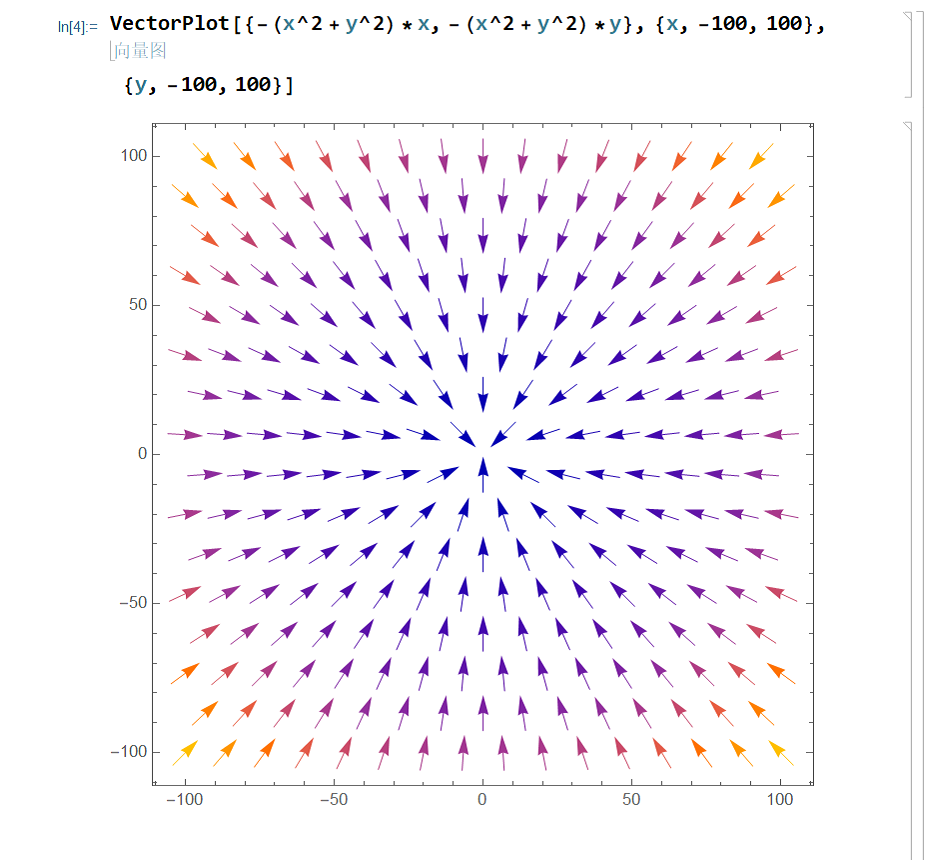
\includegraphics[width = 5cm]{3.png}
    }
    \subfigure[Plot of (b)]{
    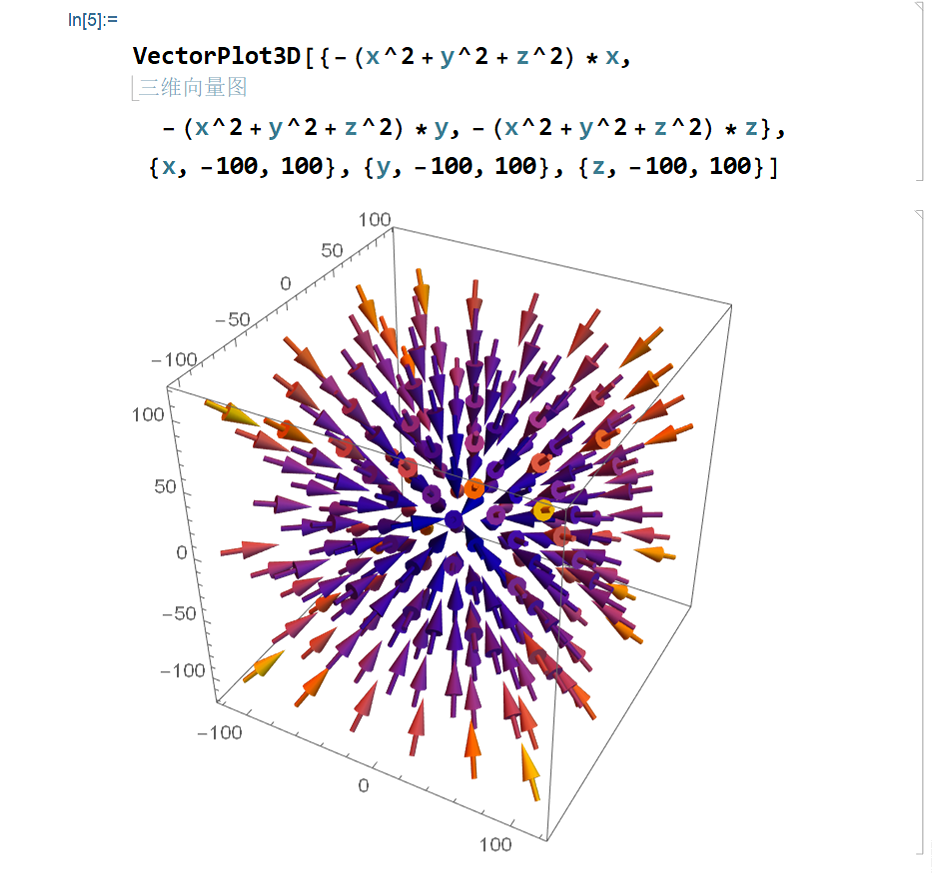
\includegraphics[width = 5cm]{4.png}
    }
\end{figure}
\begin{figure}[H]
    \centering
    \subfigure[Plot of (c) - 2D]{
    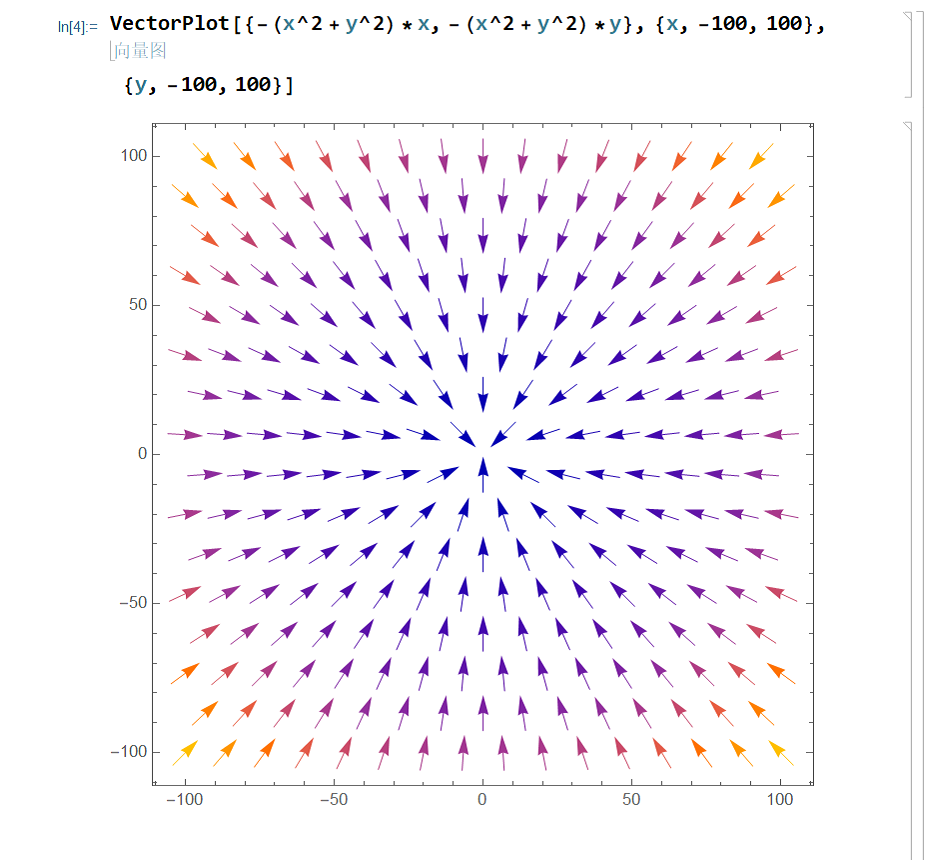
\includegraphics[width = 5cm]{3.png}
    }
    \subfigure[Plot of (c) - 3D]{
    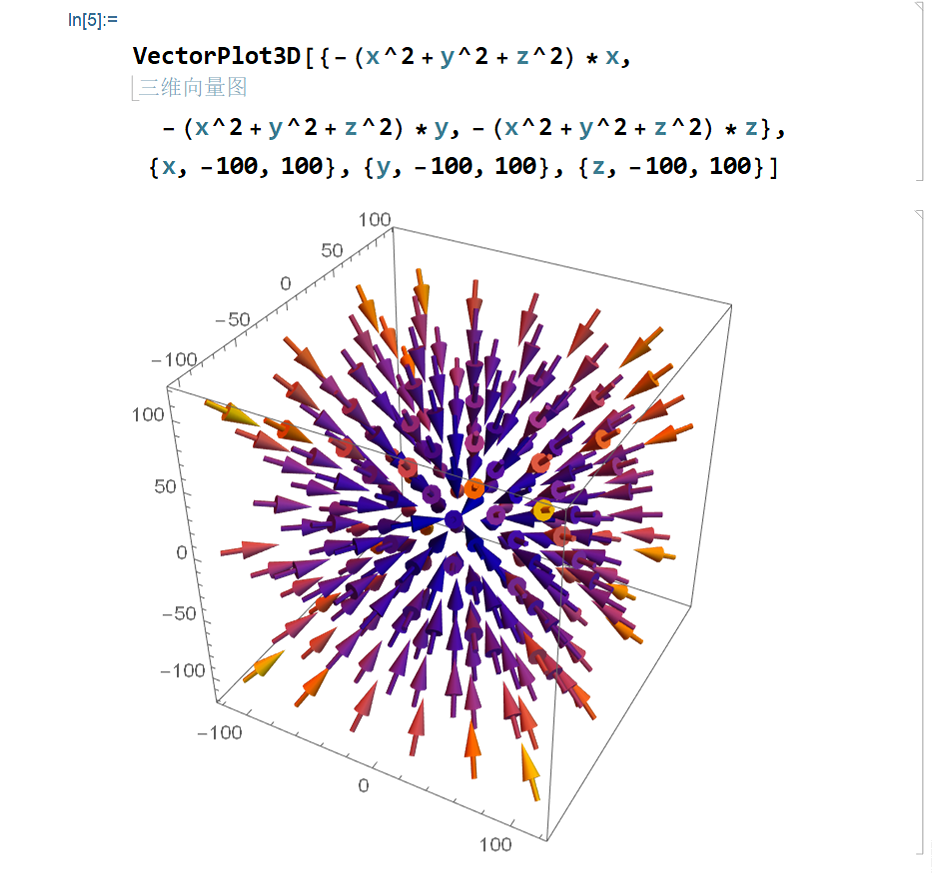
\includegraphics[width = 5cm]{4.png}
    }
\end{figure}
\begin{figure}[H]
    \centering
    \subfigure[Plot of Problem 6(A)]{
    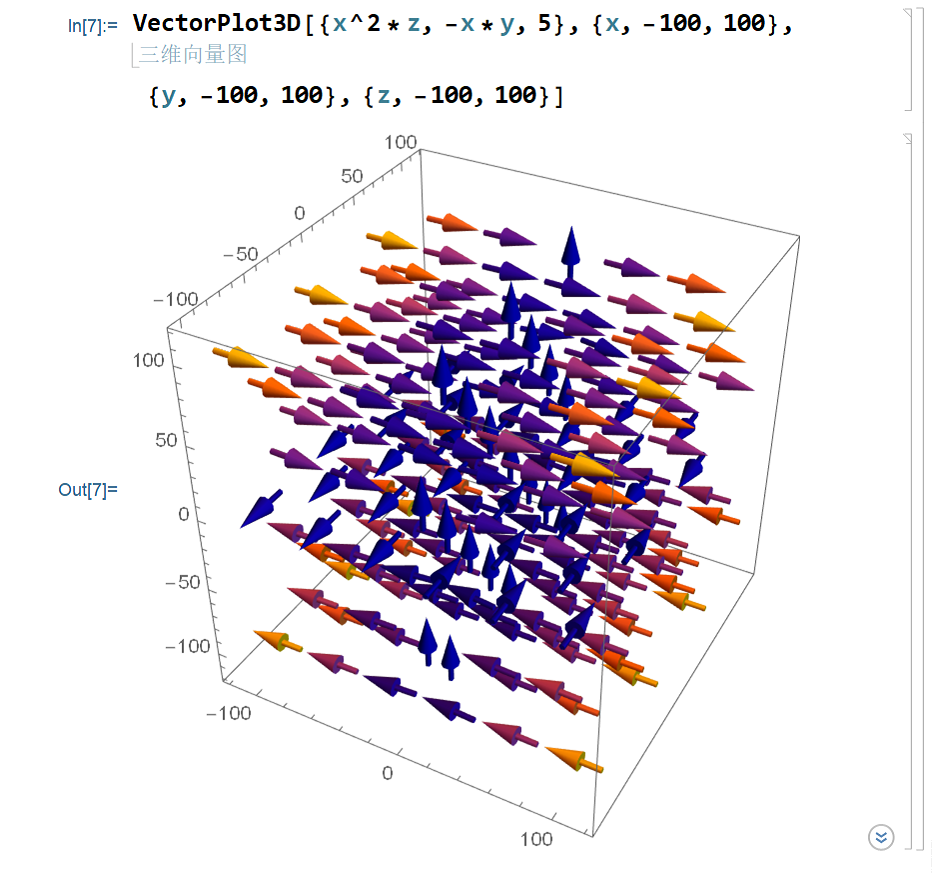
\includegraphics[width = 4.5cm]{5.png}
    }
    \subfigure[Plot of Problem 6(B)]{
    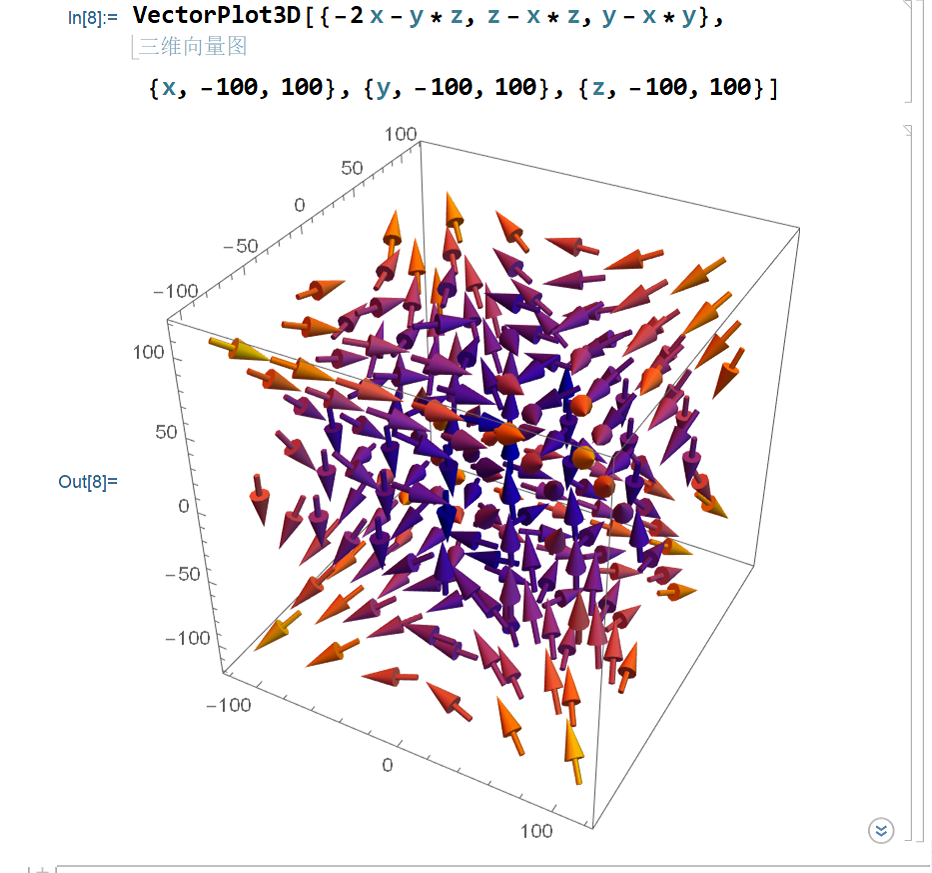
\includegraphics[width = 4.5cm]{6.png}
    }
    \caption{Plots in Problem 7}
\end{figure}
\end{document}